% Chapter 1

\chapter{Theory} % Main chapter title

\label{Chapter2} % For referencing the chapter elsewhere, use \ref{Chapter1} 

This chapter outlines the theoretical aspects of this project, covering both the linear wave theory used in the wave model and the theory of the data assimiliation methods used. The aim of the chapter is to describe all the theory required to understand the methods used in this project.

\section{Ocean Waves}

Ocean waves are a distinctive visual feature of the ocean surface, and very important to offshore operations such as wind farms. This section will describe some of the physical processes influencing ocean waves, as well as the theory of linear waves and wave energy spectra as as modelled by the WAVEWATCH III (WW3) model used in this project.

<<<<<<< HEAD

\comment{}{Here some lines need to be added informing the reader about what this chapter covers and what the aims are of this chapter.}

\section{Linear Wave Theory}\comment{}{This section is too short. In my view three topics should be discussed. 1) A short qualitative discussion of the processes that create and destroy waves and influence their propagation backed up by references. 2) The linear wave theory for propagation on which WWIII is based. This is already largely there. 3) The link between linear wave theory and the energy spectra that are modelled of WWIII. Make sure to link those spectra to the quantities we are working with (Hs, Tm01, Tm02).}

Ocean waves are a distinctive visual feature of the ocean surface\remove{,} and very important to offshore operations such as wind farms. They are an instance of surface gravity waves. This section will outline the \comment{linear wave theory}{It should be made clear that this is an approximation. Higher-order wave theories like Stokes and cnoidal waves exist, but are treated here as WWIII is based on linear wave theory.} relevant to this project, as derived in \parencite[page 253]{vallis_atmospheric_2017}\remove{, page 253}.

Parameters describing surface gravity waves include the wavenumber $k$\replace{ and}{,} direction $\theta$, and the frequency $\omega$. The first two describe the wave vector \comment{$\mathbf{k}$}{You better create a separate command for vectors and matrices. This ensures that you don't have to plough through the whole text if you want to change the format for vectors}, which has magnitude \comment{$k$ and direction $\theta$}{Add $\mathbf{k}=k \cos \theta \hat{\mathbf{x}}+ k \sin \theta \hat{\mathbf{y}}$ in which you clearly define what are directions of $\hat{\mathbf{x}}$ and $\hat{\mathbf{y}}$ as well as the definition of $\theta$}. $\omega$ here denotes the absolute frequency measured in a fixed frame of reference. If the medium is subject to currents, this will differ from the relative frequency $\sigma$ measured in a frame of reference moving with the mean current, due to the \replace{d}{D}oppler effect. This difference is quantified by the equation
=======
\subsection{Physical Processes}

Ocean waves are an instance of surface gravity waves, meaning they propagate on the interface between two fluids of different densities. Their restoring force is gravity. The focus of this project is on waves with periods from ~10s - ~0.25s, which are generated by wind, although ocean waves can exist on a wide range of scales and be influenced by other factors such as surface tension and local air pressure variations (\cite{Holthuijsen2007}, pp. 3-7).

There are multiple hypothesised physical mechanisms for the generation of waves by wind (e.g. ...). The approach from miles is poular, and described in detail in \citet{Janssen2004}, chapter 3. Qualitatively speaking, miles hypothesises that waves are generated by instability induced by the velocity shear between the air and ocean. Wind-generated waves will propagate in the same direction as the wind that generated them and will be of larger amplitude when the wind is stronger. (check)

The wind almost always acts as a source of wave energy, so there has to be a process present to dissipate waves and act as an energy sink. These processes are porrly understood but \citet{Janssen2004}, section 4.9 describes multiple physical mechanisms which may contribute to wave dissipation. One important process affecting dissipation is wave breaking, which occurs in shallow waters near shorelines. Water's molecular viscosity can lead to the damping of shorter waves and larger waves can be damped by the surface eddies induced by wave breaking.

Ocean waves in deep water are dispersive, and waves with longer wavelengths travel faster than waves with shorter wavelengths (equations \ref{eqn:disprel}-\ref{eqn:gspeed}). This leads to a phenomenon known as swell, which is the name gien to long waves that have travelled far from their source. Due to dispersion these waves have no short-wavelength component, so swell waves have longer wavelengths and periods than waves near the site of generation (known as wind sea). The other feature of swell waves is their regular appearance. While a wind sea has wave components in many different directions, by the time the waves have travelled away from the source these different components will spread out so that they do not overlap, and the resulting swell will be almost unidirectional. See figure \ref{fig:windandswell} for a schematic.

\begin{figure}
\centering
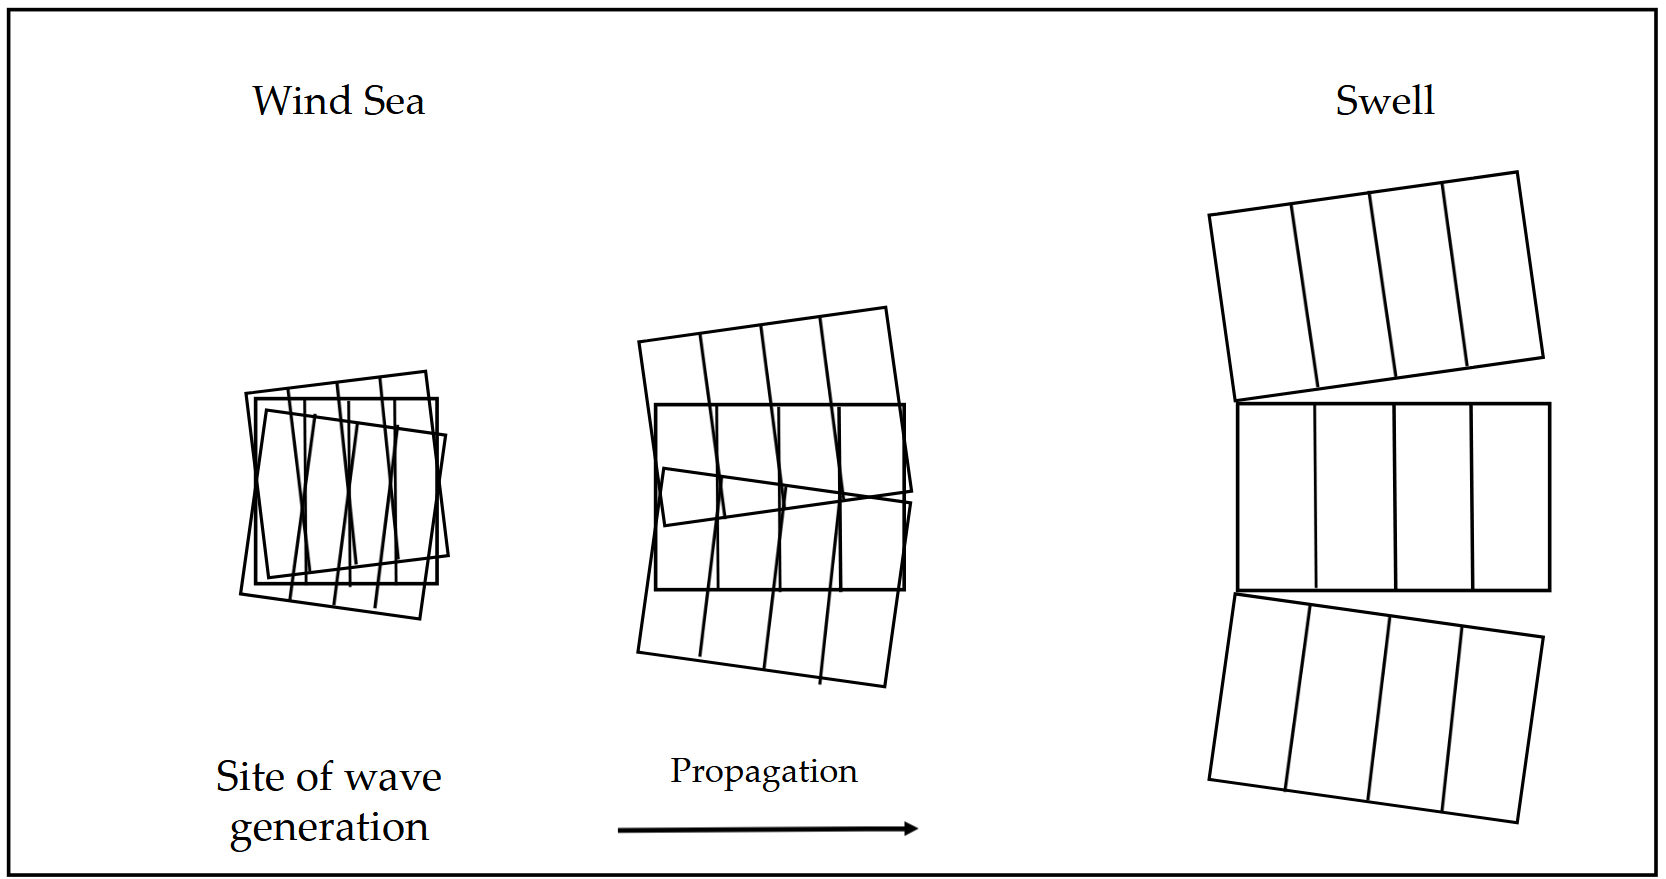
\includegraphics[width = 0.8\textwidth]{Figures/windandswell}
\caption{Schematic of the generation of wind and swell waves.}
\label{fig:windandswell}
\end{figure}

\subsection{Linear Wave Theory}

This section will outline the linear wave theory relevant to this project, as derived in \citet{Vallis2017}, page 253. Linear wave theory is an approximation, and other higher-order theories of surface gravity waves exist, such as Stokes waves (cite) and cnoidal waves (cite). These higher-order theories will not be considered here since the WAVEWATCH III model used in this project models the ocean surface as a linear superposition of simple linear waves.

Parameters describing linear waves include the wavenumber $k$, direction $\theta$ and frequency $\omega$. The first two describe the wave vector $\vect{k}$, which has magnitude $k$ and direction $\theta$ i.e. 

\begin{equation}
\vect{k} = k \cos \theta \uvec{\i} + k \sin \theta \uvec{\j}
\end{equation}

where $\uvec{\i},\uvec{\j}$ are unit vectors pointing East and North respectively. This means that $\theta$ is the angle between $\vect{k}$ and $\uvec{\i}$, measured anticlockwise from $\uvec{\i}$. $\omega$ here denotes the absolute frequency measured in a fixed frame of reference. If the medium is subject to currents, this will differ from the relative frequency $\sigma$ measured in a frame of reference moving with the mean current, due to the Doppler effect. This difference is quantified by the equation
>>>>>>> a3d2843ee1476afe2df345533f6f93a6baafad39

\begin{equation}
    \omega = \sigma + \vect{k} \cdot \vect{U}
    \label{eqn:doppler}
\end{equation}

and $\sigma$ and $k$ are related by the dispersion relation

\begin{equation}
    \sigma^2 = gk\tanh{kD}
    \label{eqn:disprel}
\end{equation}

The dispersion relation has two limiting forms:

\begin{itemize}
    \item Deep water waves, where $kD \gg 1$, so $\tanh{kD} \approx 1$ and $\sigma^2 \approx gk$.
    \item Shallow water waves, where $kD \ll 1$, so $\tanh{kD} \approx kD$ and $\sigma^2 \approx gk^2D$
\end{itemize}

The phase speed is then given by

\begin{equation}
c = \frac{\sigma}{k} \approx \begin{cases}
            \sqrt{\frac{g}{k}} &\text{in deep water} \\
            \sqrt{gD} &\text{in shallow water}
\end{cases}
\label{eqn:pspeed}
\end{equation}

and the \comment{group speed}{Explain the physical relevance of the group speed vs the phase speed} may be expressed as

\begin{equation}
c_g = \frac{\partial\sigma}{\partial k} = \frac{1}{2}c \left(1 + \frac{2kD}{\sinh{2kD}} \right) \approx \begin{cases}
    \frac{1}{2} c &\text{in deep water} \\
    c &\text{in shallow water}
\end{cases}
\label{eqn:gspeed}
\end{equation}

The phase speed is the speed at which the wave peaks and troughs move, whereas the group speed is the speed at which wave groups move. The group speed is then the speed at which energy is transported by the wave. The wave travels in the direction of the wave vector $\vect{k}$ so the group and phase velocities are given by

\begin{align*}
\vect{c}& = c \cos \theta \uvec{\i} + c \sin \theta \uvec{\j} \\
\vect{c}_g& = c_g \cos \theta \uvec{\i} + c_g \sin \theta \uvec{\j}
\end{align*}

We can now use scale analysis to see that $\omega$ and $\sigma$ generally have similar values. The ratio between $\vect{k}\cdot\vect{U}$ and $\sigma$ in equation \ref{eqn:doppler} is

\[
\frac{\vect{k}\cdot\vect{U}}{\sigma} \sim \frac{kU}{\sigma} = \frac U c
\]

Where $U = |\vect{U}|$ is the mean current speed. Since $c \gg U$ in general, this ratio is small and so $\omega \approx \sigma$.

\subsection{Wave Spectra}
\label{sec:wavespectra}

Note that equations \ref{eqn:doppler} - \ref{eqn:gspeed} are valid for linear waves of a single frequency and direction. Real ocean waves are more complicated than this, containing multiple frequencies propagating in multiple directions. The WAVEWATCH III model used in this project models ocean waves as a superposition of these simple linear waves.

Surface waves with multiple frequencies and directions are represented using a wave spectrum $F = F(\sigma,\theta)$, which is also a function of position and time. $F$ represents the sea surface height variance associated with a particular frequency $\sigma$ and direction $\theta$, so the total height variance is 

\begin{equation}
\overline{\eta^2} = \iint F d\sigma d\theta
\label{eqn:waveenergy}
\end{equation}

This is related to the wave energy via $E = \rho g \overline{\eta^2}$. A rigourous definition of $F$ is given in \citet{Holthuijsen2007}, section 3.5.6. One can also define the unidirectional spectrum $S(\sigma) = \int F(\sigma,\theta) d\theta$ which quantifies the surface height variance as a function of frequency. This can be integrated to calculate the energy contained in a specific frequency band $\Delta \sigma$:

\begin{equation}
\Delta E = \int_{\Delta \sigma} S(\sigma) d\sigma
\end{equation}

$S$ is a helpful diagnostic from which information about the appearance of the waves can be inferred. A widely spread spectrum implies irregular waves with many different frequency components whereas a tight spectrum implies regular waves with one dominant frequency. Low frequency waves correspond to swell, while high frequency waves correspond to a wind sea. An example of a unidirectional spectrum is plotted in figure \ref{fig:examplespec}.

\begin{figure}
\centering
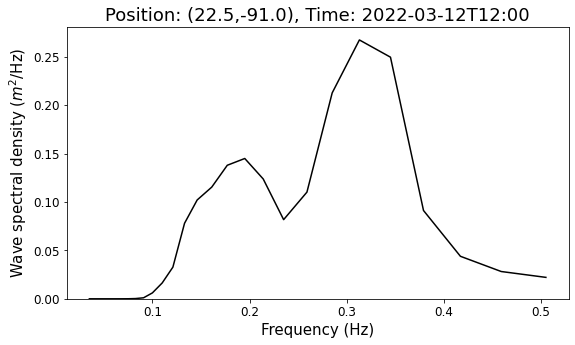
\includegraphics[width = 0.7\textwidth]{Figures/examplespec}
\caption{An example unidirectional spectrum from a point in the gulf of Mexico. Calculated from WW3 spectral forecast data.}
\label{fig:examplespec}
\end{figure}

Here, we also define the wave spectral moments which are derived from the unidirectional spectrum:

\begin{equation}
m_k = \int S(\sigma) \sigma^k d\sigma, m = \dots,-1,0,1,\dots
\label{eqn:moments}
\end{equation}

<<<<<<< HEAD
These moments can be used to derive other important wave variables, such as significant wave height and dominant wave period, from the spectrum (expand). \comment{Finally we define the wave action}{This better moves to the paragraphs on linear wave theory.}
=======
Note that $m_0 = \overline{\eta^2}$ is the overall surface height variance. These moments can be used to derive other important wave variables from the spectrum, such as significant wave height and wave period. In this project we focus on the significant wave height Hs and two measures of frequency Tm01, Tm02. These variables are defined below in equation \ref{eqn:mainvars} (expand?).

\begin{align}
\text{Hs} &= 4\sqrt{m_0} \\
\text{Tm01} &= \frac{m_0}{m_1} \\
\text{Tm02} &= \sqrt{\frac{m_0}{m_2}}
\label{eqn:mainvars}
\end{align}

 Finally we define the wave action
>>>>>>> a3d2843ee1476afe2df345533f6f93a6baafad39

\[
N(\sigma,\theta) = \frac {F(\sigma,\theta)} {\sigma}
\]

$N$ is conserved in the absence of sources and sinks \parencite{Bretherton1968}, so it very useful for wave modelling. WW3 works by evolving the wave action according to the action of sources and sinks (see section \ref{sec:model}).

\section{Data Assimilation}\comment{}{Strictly speaking we are using the update step of the ETKF which is somewhat unusually. This section can be used to show that this approach is in absence of localization and with a linear operator is equivalent to the weak 4DEnVar.}

As well as the model, we also have some direct observations of the waves which we would like to make use of to improve our predictions. \comment{We use techniques of data assimilation to achieve this.}{Add general explanation what DA is doing. I.e. finding estimates that lie closer to truth using the information in the observations.}

<<<<<<< HEAD
We take a vector $\x \in \mathbb{R}^n$ to represent \comment{the state of the system}{Extend the description of how $\x$ is related to the model}, assuming it has a normal background distribution \comment{$\x \sim N(\x_b,\mathbf{B})$}{}. We take a vector $\y \in \mathbb{R}^p$ to represent a set of observations, and assume $\y$ is related to $\x$ via an observation operator $\mathcal{H}: \mathbb{R}^n \rightarrow \mathbb{R}^p$:
=======
\subsection{Vector Representations and Cost Function}

We take a vector $\x \in \mathbb{R}^n$ to represent the state of the system, assuming it has a normal background distribution $\x \sim N(\x_b,\mat{B})$. We take a vector $\y \in \mathbb{R}^p$ to represent a set of observations, and assume $\y$ is related to $\x$ via an observation operator $\mathcal{H}: \mathbb{R}^n \rightarrow \mathbb{R}^p$:
>>>>>>> a3d2843ee1476afe2df345533f6f93a6baafad39

\comment{}{It might be better to introduce $\x_{true}$ here to make a distinction between a specific value of the state and reference to the state in general.}
\[
\y = \mathcal{H}(\x) + \varepsilon
\]

where the error term $\varepsilon$ is assumed to be normally distributed with mean zero and covariance $\mat{R}$: $\varepsilon \sim N(0,\mat{R})$. We call the vector spaces containing $\x$ and $\y$ the state space and observation space respectively. In operational contexts, the dimensions of these spaces are very large: typically $n \sim 10^8$ and $p \sim 10^6$. This means that considerable computational resources are required in most cases and computational efficiency is a key consideration in any operational DA implementation.

<<<<<<< HEAD
In our case $\mathcal{H}$ is linear i.e. there is a matrix $\mathbf{H} \in \mathbb{R}^{n \times p}$ such that $\mathcal{H}(\x) = \mathbf{H}\x$\remove{,} and so $\prob(\y|\x) = N(\mathbf{H}\x,\mathbf{R})$. We can then express the distribution of $\x$ given some set of observations $\y$ using Bayes' theorem:
=======
In our case $\mathcal{H}$ is linear i.e. there is a matrix $\mat{H} \in \mathbb{R}^{n \times p}$ such that $\mathcal{H}(\x) = \mat{H}\x$, and so $\prob(\y|\x) = N(\mat{H}\x,\mat{R})$. We can then express the distribution of $\x$ given some set of observations $\y$ using Bayes' theorem:
>>>>>>> a3d2843ee1476afe2df345533f6f93a6baafad39

\begin{equation}
    \prob(\x|\y) = \prob(\y|\x) \frac{\prob(\x)}{\prob(\y)}
\end{equation}

This allows $\prob(\x|\y)$ to be determined since $\prob(\y|\x)$ and $\prob(\x)$ are known, and $\prob(\y)$ is independent of $\x$ so it acts as a normalisation constant. Since all the distributions involved are normal, $\prob(\x|\y)$ will be normally distributed also:

\comment{}{You need define $\sim$ here.}
\begin{equation}
    \prob(\x|\y) \sim e^{-\frac 1 2 \left( \norm[\mat{B}^{-1}]{\x - \x_b}^2 + \norm[\mat{R}^{-1}]{\y - \mat{H}\x}^2\right)}
\end{equation}

adopting the notation $\norm[\mat{M}]{\vect{a}}^2 = \vect{a}^\top \mat{M} \vect{a}$. Finding the most likely value of $\x$ given this distribution is equivalent to minimising a cost function

\begin{equation}
    J(\x) = \frac 1 2 \norm[\mat{B}^{-1}]{\x - \x_b}^2 + \frac 1 2 \norm[\mat{R}^{-1}]{\y - \mat{H}\x}^2
    \label{eqn:cost3d}
\end{equation}

<<<<<<< HEAD
The state that minimises this cost function is called the analysis $\x_a$ and \comment{may be expressed as}{reference needed and $d^o_b$ should be a bold vector}
=======
The first term of \ref{eqn:cost3d} represents the deviation of $\x$ from the background state and the second term represents the deviation from the observations, with the overall cost function being a sum of these two weighted by the background and observation error matrices. This means that when the background error is large compared to the observational error, the observations will be given more weight and vice versa.

\subsection{Kalman Filters}

The state that minimises this cost function is called the analysis $\x_a$ and may be expressed as
>>>>>>> a3d2843ee1476afe2df345533f6f93a6baafad39

\begin{equation}
    \x_a = \x_b + \mat{K}\vect{d}^o_b
\label{eqn:analysisupdate}
\end{equation}

<<<<<<< HEAD
where $d^o_b = \y - \mathbf{H}\x$ is the innovation and $\mathbf{K} = \mathbf{B}\mathbf{H}^\top\left(\mathbf{H}\mathbf{B}\mathbf{H}^\top + \mathbf{R}\right)^{-1}$ is the Kalman gain. Note that the increment $d^a_b = \x_a - \x_b$ is given by  $ \mathbf{B}\left(\mathbf{H}^\top\left(\mathbf{H}\mathbf{B}\mathbf{H}^\top + \mathbf{R}\right)^{-1} d^o_b \right)$, so it always lies in the column space of $\mathbf{B}$. This means that $\mathbf{B}$ is crucial to determining how information from the observations is spread around the domain by the DA system. In particular, if $\mathbf{B}$ is rank deficient, then all possible increments lie within a strict subspace of the state space. \comment{(so?)}{Limits the degrees of freedom of the DA corrections.}

\comment{}{I don't think the remaining part of this section is relevant as there is no prediction step in our setup. Introduction of the ensemble estimate of $\mathbf{B}$, the analysis mean and analysis covariance would be beneficial at this point.}
In most contexts, observations are not all simultaneous \add{assimilated} but instead come from a sequence of times $t = 0,1,\dots$. One approach to assimilating non-simultaneous observations is to use a filter method such as the Ensemble Kalman Filter \parencite{Evensen1994,Houtekamer1998,Anderson2001}. A filter method consists of successive analysis steps, in which the observations from time $t$ are assimilated according to equation \ref{eqn:analysisupdate}, alternating with update steps, in which the forecast model is used to evolve the state forward to time $t+1$.
=======
where $\vect{d}^o_b = \y - \mat{H}\x$ is the innovation and $\mat{K} = \mat{B}\mat{H}^\top\left(\mat{H}\mat{B}\mat{H}^\top + \mat{R}\right)^{-1}$ is the Kalman gain (derived in \cite{Asch2016}, pp. 92-96). Note that the increment $\vect{d}^a_b = \x_a - \x_b$ is given by $ \mat{B}\left(\mat{H}^\top\left(\mat{H}\mat{B}\mat{H}^\top + \mat{R}\right)^{-1} \vect{d}^o_b \right)$, so it always lies in the column space of $\mat{B}$. This means that $\mat{B}$ is crucial to determining how information from the observations is spread around the domain by the DA system. In particular, if $\mat{B}$ is rank deficient, then all possible increments lie within a strict subspace of the state space. This reduces the degrees of freedom in the corrections the DA system can make, which limits the performance of the system.

DA methods which use equation \ref{eqn:analysisupdate} are called Kalman filters, in which context it is called the analysis step. Kalman filters generally alternate this analysis step with a forecast step in which a forecast model is used to evolve the state forward to the next observation time. In this project we do not have access to the forecast model, so we will only make use of the analysis step to update the state.
>>>>>>> a3d2843ee1476afe2df345533f6f93a6baafad39

The specific method we will use is called the ensemble transform Kalman filter (ETKF) in which the analysis is performed in ensemble subspace rather than in the state space. Algebraically this means expressing the increment as a linear combination of ensemble perturbations

\begin{align}
\mat{X}_f &= \frac{1}{\sqrt{N- 1}} \left( \x^f_1 - \overline{\x}^f, \x^f_2 - \overline{\x}^f, \dots, \x^f_N - \overline{\x}^f \right) \\
\x^a &= \overline{\x}^f + \mat{X}_f \vect{w}^a
\end{align}

Where $\x^f_i$ is the state of ensemble member $i$ prior to assimilation and the ensemble mean $\overline{\x}^f$ is used as the background state. From \citet{Asch2016} pp.163-164, the optimal coefficient vector $\vect{w}^a$ is given by

\begin{equation}
\vect{w}^a = \left( \mat{I}_N + \mat{X}_f^\top \mat{H}^\top \mat{R}^{-1} \mat{H} \mat{X}_f \right) ^{-1} \mat{X}_f^\top \mat{H}^\top \mat{R}^{-1} \vect{d}^o_b
\label{eqn:ETKFinc}
\end{equation}

This method is algebraically equivalent to working in state space with the background error covariance matrix given by the foreccast error covariance matrix

\begin{equation}
\mat{P}_f = \mat{X}_f \mat{X}_f^\top
\label{eqn:ferrorcov}
\end{equation}

This matrix is rank deficient since its column space has dimension equal to the ensemble size, but working in ensemble space has considerable advantages over working in state space in terms of computational cost \parencite{Hunt2007}. The full analysis ensemble can then be generated from the analysis state derived in equation \ref{eqn:ETKFinc} via

\begin{equation}
\x^a_i = \x^a + ...
\label{eqn:ETKFens}
\end{equation}

And the analysis error covariance $\mat{P}_a$ can be defined similarly to $\mat{P}_f$ but from the analysis ensemble:

\begin{align}
\mat{X}_a &= \frac{1}{\sqrt{N- 1}} \left( \x^a_1 - \x^a, \x^a_2 - \x^a, \dots, \x^a_N - \x^a \right) \\
\mat{P}_a &= \mat{X}_a \mat{X}_a^\top
\end{align}

Another advantage of the ETKF (compared to the stochastic ensemble Kalman filter) is that $\mat{P}_a$ matches exactly the form given by Kalman theory (cite?)

\subsection{Practical Aspects}
\label{sec:DApractice}

When calculating $\mat{P}^f$ from the ensemble, spurious covariances may arise at long distances, especially when the ensemble size is small. This is problematic as it can lead to large increments far from observation locations, which is physically unrealistic. One way to fix this is called localisation, and involves multiplying each component of the background error matrix $\mat{P}^f_{ij}$ by a factor which depends on the distance between gridpoints $i$ and $j$. Representing this distance with $d(i,j)$, we have the following equation:

\begin{equation}
\mat{P}^{f\prime}_{ij} = \mat{P}^f_{ij} f(d(i,j))
\end{equation}

The function $f$ should be close to 1 when $d(i,j)$ is small and close to 0 when $d(i,j)$ is large, to suppress covariances at long distances while allowing them to exist at short distances (FIND SOURCE)

Another problem that may be encountered is... (filter divergence - tailor to our case)

PROOF OF EQUIVALENCE WITH WEAK 4DENVAR

\textbf{EnKF description - may not be needed}

In most contexts, observations are not all simultaneous but instead come from a sequence of times $t = 0,1,\dots$. One approach to assimilating non-simultaneous observations is to use a filter method such as the Ensemble Kalman Filter \parencite{Evensen1994,Houtekamer1998,Anderson2001}. A filter method consists of successive analysis steps, in which the observations from time $t$ are assimilated according to equation \ref{eqn:analysisupdate}, alternating with update steps, in which the forecast model is used to evolve the state forward to time $t+1$.

Where $N$ is the ensemble size, $\x_t^{(i)}$ is the state of ensemble member $i$ before the analysis step at time $t$ and $\overline{\x}_t = \frac{1}{N} \Sigma_{i=1}^{N} \x_t^{(i)}$ i.e. the ensemble mean.

In general, the observations from each time $t$ may be available at different locations, or observations of different variables may be available, so the observation operator and observation error covariance matrix are functions of time. Denoting these at time $t$ by $\mat{H}_t, \mat{R}_t$, the Kalman gain matrix takes the form

\[
\mat{K}_t = \mat{P}^f_t\mat{H}_t^\top\left(\mat{H}_t\mat{P}^f_t\mat{H}_t^\top + \mat{R}_t\right)^{-1}
\]

The EnKF method is prone to a problem called filter divergence -  sampling error in the calculation of $\mat{P}^f_t$ means the magnitude of the forecast error covariance tends to erroneously shrink over time \parencite{Jazwinski1970}. This means that after some time, the ensemble distribution becomes very tight and further observations do not affect the state of the ensemble, resulting in forecast analysis states which diverge from the true state. (schematic) To counteract this, we will employ the method of inflation described in \cite{Anderson1999}, where the forecast error covariance matrix is multiplied by a factor $\alpha$ before the analysis step is performed.

\subsection{(Description of 4DEnVar - may not be needed)}

In our case, we have observations from multiple times $t = 0,1,\dots,T$ spread out over some time window, and we expect the state $\x$ to evolve over this time window. This evolution may be predicted using the model as follows: let $\x_0$ represent the state of the system at $t=0$, then we define the model operator $\mathcal{M}_t$ for each $t$ such that $\x_{t+1} = \mathcal{M}_t\left(\x_t\right)$ as predicted by the model. The cost function then becomes

\begin{align}
	J\left(\x_0\right) &= \frac 1 2 \norm[\mat{B}_0^{-1}]{\x_0 - \x_b}^2 + \frac 1 2 \sum_{t=0}^T \norm[\mathbf{R}_t^{-1}]{\y_t - \mathbf{H}_t\x_t}^2 \\
	&= \frac 1 2 \norm[\mathbf{B}_0^{-1}]{\x_0 - \x_b}^2 + \frac 1 2 \sum_{t=0}^T \norm[\mathbf{R}_t^{-1}]{\y_t - \mathbf{\hat{h}}_t\x_0}^2
\end{align}

where the observations $\y_t$ and matrices $\mathbf{H}_t,\mathbf{R}_t$ are valid at time $t$, \comment{and}{$\hat{h}_{t}$ is an operator and should therefore be capitalized} $\mathbf{\hat{h}}_t = \mathbf{H}_t\mathcal{M}_{0 \rightarrow t}$ using the abbreviation $ \mathcal{M}_{0 \rightarrow t} = \mathcal{M}_{t-1}\mathcal{M}_{t-2}\dots\mathcal{M}_0$.

We will use the 4DEnVar method, where a control variable transform is used to write $\x_0$ as a linear combination of the ensemble perturbations:

\begin{align*}
	\overline{\x}_b &= \frac 1 N \sum_{n=1}^N \x_b^{(n)} \\
	\mathbf{X}'_b &= \frac{1}{\sqrt{N- 1}} \left( \x_b^{(1)} - \overline{\x}_b, \x_b^{(2)} - \overline{\x}_b, \dots, \x_b^{(N)} - \overline{\x}_b \right) \\
	\x_0 &= \overline{\x}_b + \mathbf{X}'_b \mathbf{\chi}
\end{align*}

Here $\x_b^{(n)}$ represents the background state from ensemble member $n$, and $N$ is the ensemble size. The cost function can then be rewritten in terms of $\mathbf{\chi}$ and simplified by linearising $\mathbf{\hat{h}}_t$ around $\overline{\x}_b$:

\begin{equation}
J(\mathbf{\chi}) = \frac 1 2 \norm{\mathbf{\chi}}^2 + \frac 1 2 \sum_{t=0}^T \norm[\mathbf{R}_t^{-1}]{\y_t - \mathbf{\hat{h}}_t\overline{\x}_b - \mathbf{\hat{H}}_t \mathbf{X}'_b \mathbf{\chi}}^2
\end{equation}

where $\mathbf{\hat{H}}_t = \mathbf{H}_t\mathbf{M}_{0 \rightarrow t}$ is the linearisation of $\mathbf{\hat{h}}_t$. This cost function is simplified by taking a background error covariance matrix of the form $\mathbf{B} = \mathbf{X}'_b\mathbf{X}_b^{\prime\top}$, which reduces to the identity under the control variable transform. This cost function has gradient

\[
\nabla J(\mathbf{\chi}) = \mathbf{\chi} + \sum_{t=0}^T\left(\mathbf{\hat{H}}_t \mathbf{X}'_b\right)^\top \mathbf{R}_t^{-1} \left(\mathbf{\hat{h}}_t \mathbf{X}'_b \chi + \mathbf{\hat{H}}_t \overline{\x}_b - \y_t\right)
\]

A major advantage of this formulation is that we can make the approximation

\[
\mathbf{M}_{0 \rightarrow t} \left( \x^{(n)}_b - \overline{\x}_b \right) \approx \mathcal{M}_{0 \rightarrow t} \left( \x^{(n)}_b \right) - \overline{\mathcal{M}_{0 \rightarrow t} \left( \x_b \right)}
\]

Since $\mathbf{H}_t \mathbf{M}_{0 \rightarrow t} \left( \x^{(n)}_b - \overline{\x}_b \right)$ is the $n^{\text{th}}$ column of $\mathbf{\hat{H}}_t \mathbf{X}'_b$, this approximation allows us to compute the cost function and its gradient without a tangent linear or adjoint model, which is a computationally expensive aspect of most variational data assimilation schemes \citep{Bannister2017}.

